\section{Class Diagram}

\subsection{Class diagram}

\begin{figure}[H]
    \centering
    \IfFileExists{pictures/access_control_class_diagram.png}{%
        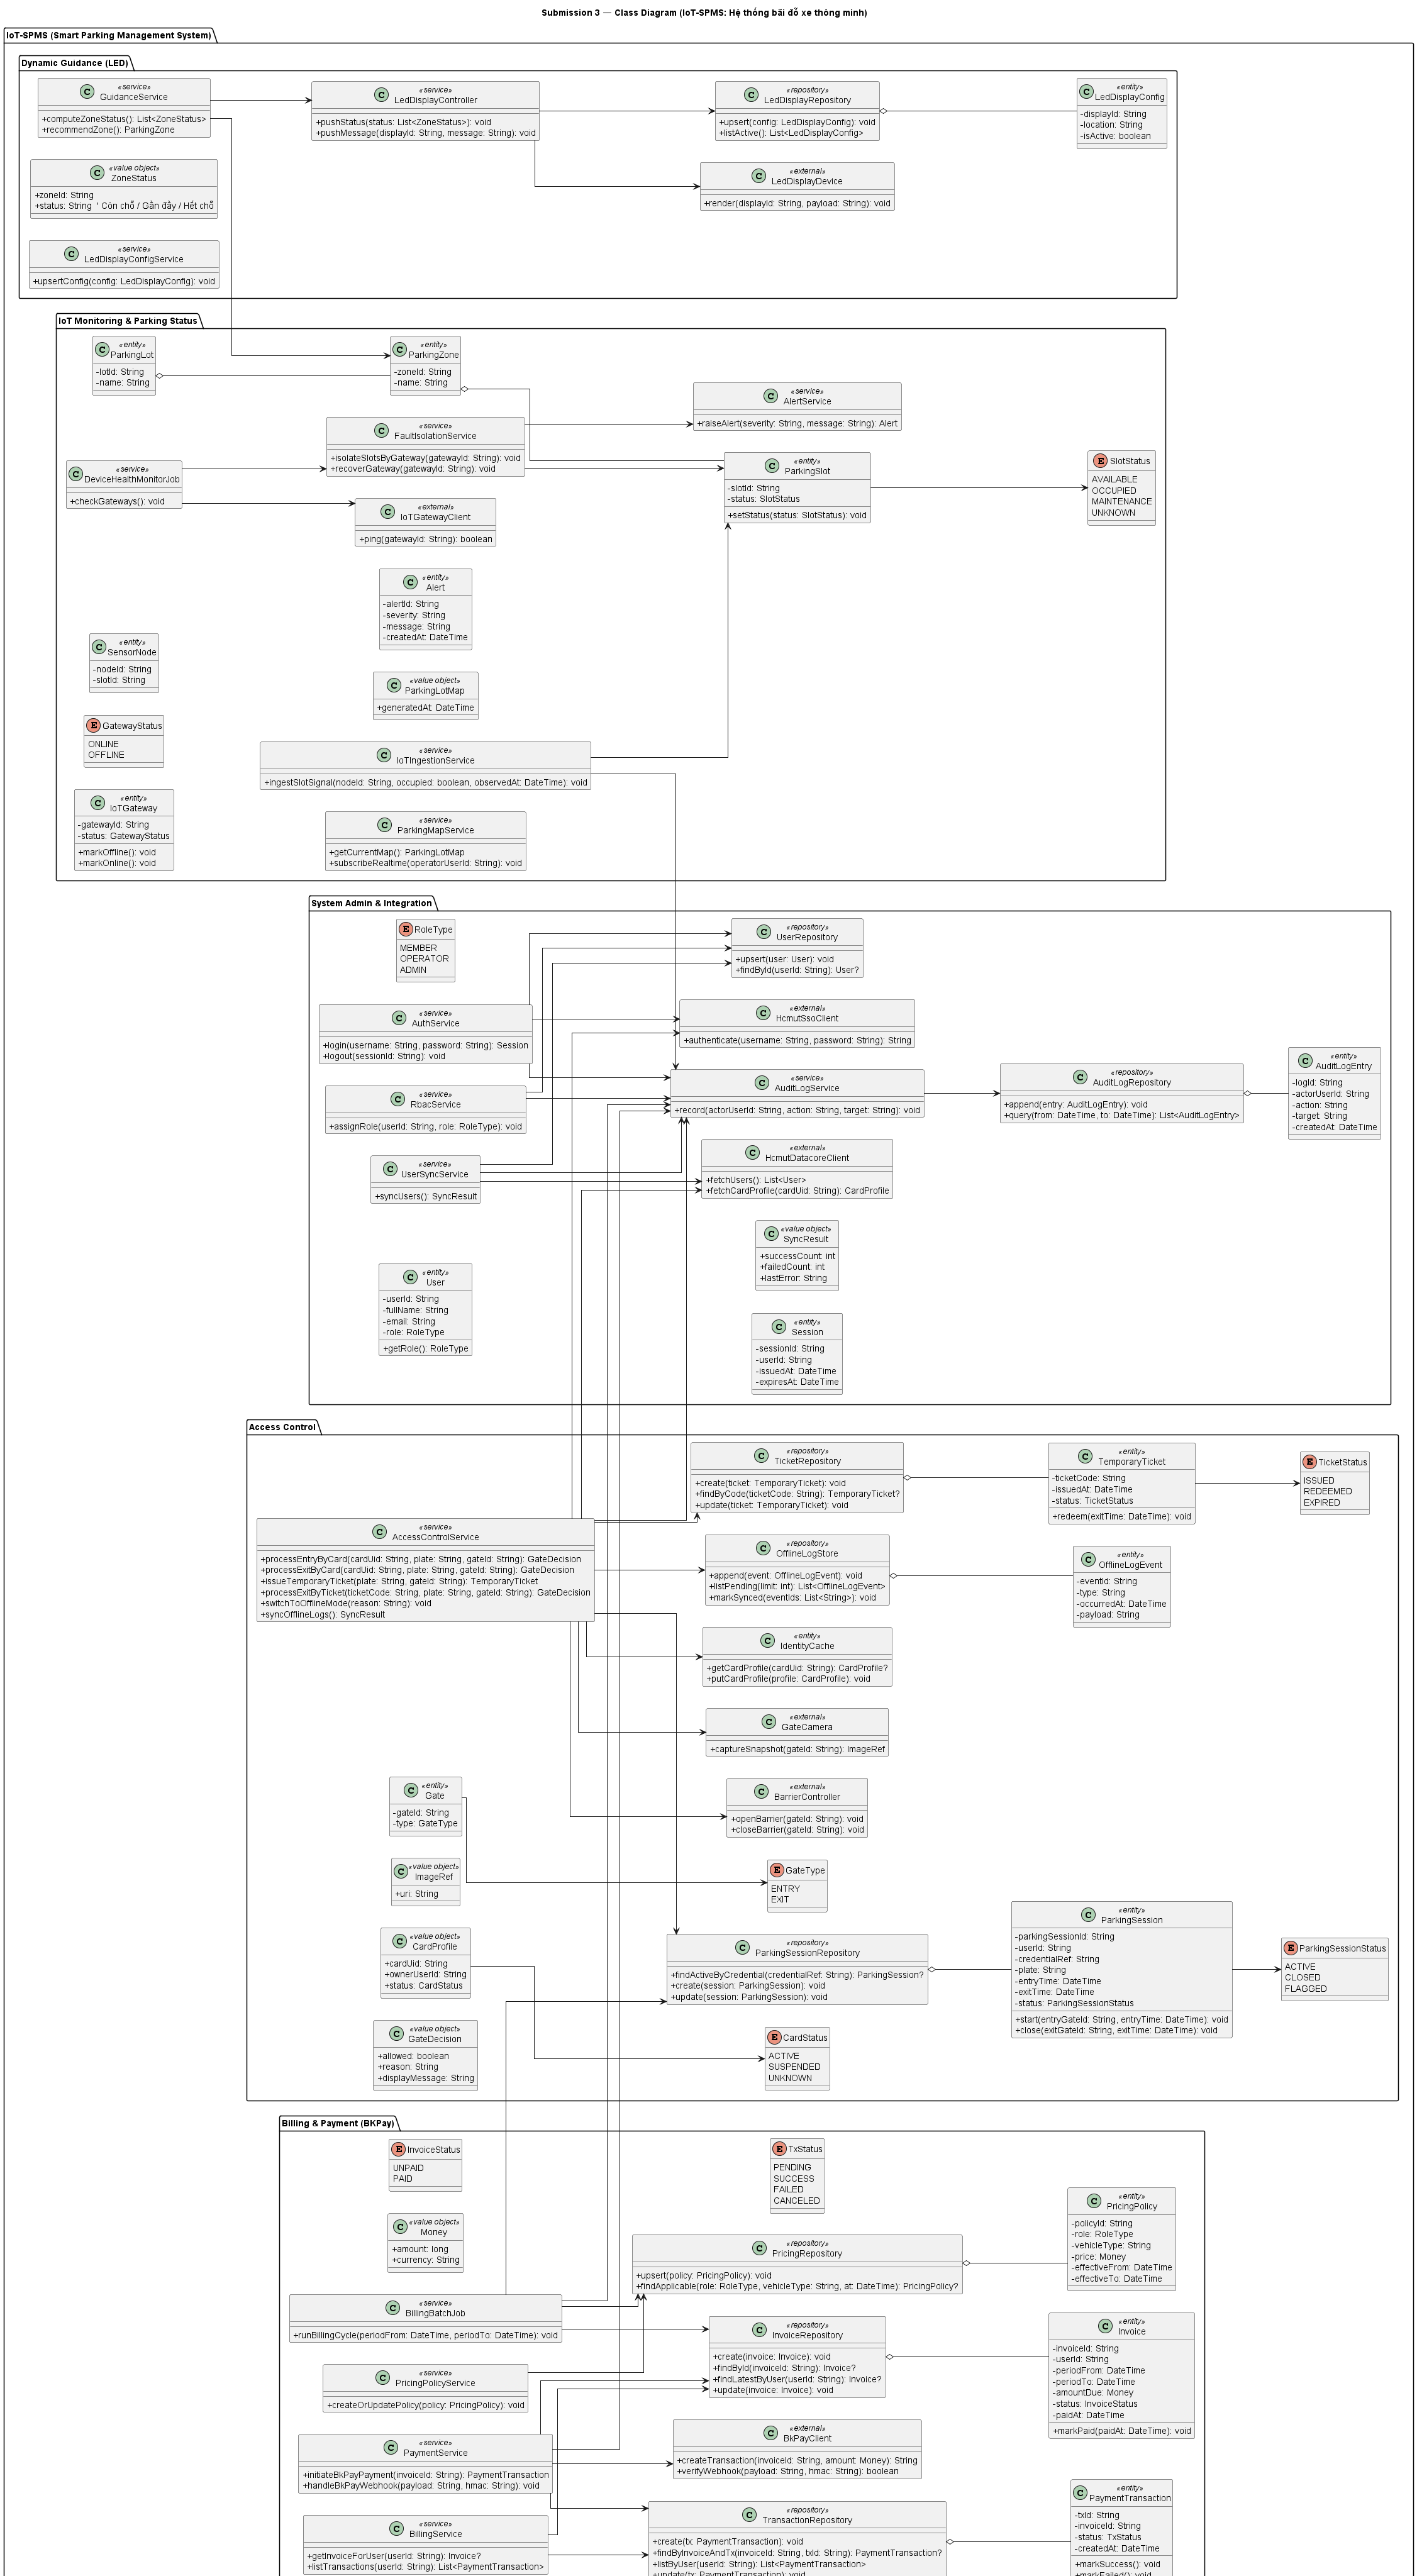
\includegraphics[width=1.15\textwidth]{pictures/access_control_class_diagram.png}
    }
    \caption{Class diagram toàn hệ thống IoT-SPMS}
    \label{fig:class-diagram-overview}
\end{figure}

\subsection{Mô tả}

\noindent\textbf{Quản trị hệ thống và tích hợp}
\begin{itemize}[leftmargin=1.5cm]
    \item \textbf{User}
    \begin{itemize}
        \item \textit{Mô tả:} Lớp người dùng nền tảng cho toàn hệ thống, lưu thông tin định danh được đồng bộ từ HCMUT\_DATACORE và role dùng cho RBAC.
        \item \textit{Thuộc tính chính:} \texttt{userId}, \texttt{fullName}, \texttt{email}, \texttt{role}, \texttt{status}, \texttt{cardUid}.
        \item \textit{Phương thức chính:} \texttt{getRole()}.
    \end{itemize}

    \item \textbf{AuthService}
    \begin{itemize}
        \item \textit{Mô tả:} Xử lý đăng nhập, đăng xuất và tạo phiên làm việc nội bộ sau khi xác thực qua HCMUT\_SSO.
        \item \textit{Phương thức chính:} \texttt{login(username, password)}, \texttt{logout(sessionId)}.
    \end{itemize}

    \item \textbf{UserSyncService}
    \begin{itemize}
        \item \textit{Mô tả:} Đồng bộ hồ sơ người dùng từ HCMUT\_DATACORE về cơ sở dữ liệu cục bộ.
        \item \textit{Phương thức chính:} \texttt{syncUsers()}.
    \end{itemize}

    \item \textbf{RbacService}
    \begin{itemize}
        \item \textit{Mô tả:} Quản lý phân quyền người dùng và gán vai trò phù hợp cho từng tác nhân trong hệ thống.
        \item \textit{Phương thức chính:} \texttt{assignRole(userId, role)}.
    \end{itemize}

    \item \textbf{UserRepository}
    \begin{itemize}
        \item \textit{Mô tả:} Tầng truy xuất dữ liệu cho thông tin người dùng nội bộ.
        \item \textit{Phương thức chính:} \texttt{upsert(user)}, \texttt{findById(userId)}.
    \end{itemize}

    \item \textbf{AuditLogService} và \textbf{AuditLogRepository}
    \begin{itemize}
        \item \textit{Mô tả:} Ghi nhận và truy vấn audit log cho các thao tác quản trị, kiểm soát ra vào và thanh toán.
        \item \textit{Phương thức chính:} \texttt{record(actorUserId, action, target)}, \texttt{append(entry)}, \texttt{query(from, to)}.
    \end{itemize}

    \item \textbf{HcmutSsoClient} và \textbf{HcmutDatacoreClient}
    \begin{itemize}
        \item \textit{Mô tả:} Hai adapter tích hợp với hệ thống bên ngoài. \texttt{HcmutSsoClient} dùng để xác thực, còn \texttt{HcmutDatacoreClient} dùng để lấy hồ sơ người dùng và thông tin thẻ ID.
        \item \textit{Phương thức chính:} \texttt{authenticate(username, password)}, \texttt{fetchUsers()}, \texttt{fetchCardProfile(cardUid)}.
    \end{itemize}
\end{itemize}

\noindent\textbf{Kiểm soát ra vào bãi đỗ}
\begin{itemize}[leftmargin=1.5cm]
    \item \textbf{AccessControlService}
    \begin{itemize}
        \item \textit{Mô tả:} Điều phối toàn bộ luồng xe vào/ra bằng thẻ ID hoặc vé tạm, đồng thời hỗ trợ chế độ offline khi mất kết nối hạ tầng.
        \item \textit{Phương thức chính:} \texttt{processEntryByCard(cardUid, plate, gateId)}, \texttt{processExitByCard(cardUid, plate, gateId)}, \texttt{issueTemporaryTicket(plate, gateId)}, \texttt{processExitByTicket(ticketCode, plate, gateId)}, \texttt{switchToOfflineMode(reason)}, \texttt{syncOfflineLogs()}.
    \end{itemize}

    \item \textbf{BarrierController}
    \begin{itemize}
        \item \textit{Mô tả:} Điều khiển đóng/mở barrier tại từng cổng vào hoặc cổng ra.
        \item \textit{Phương thức chính:} \texttt{openBarrier(gateId)}, \texttt{closeBarrier(gateId)}.
    \end{itemize}

    \item \textbf{GateCamera}
    \begin{itemize}
        \item \textit{Mô tả:} Ghi nhận ảnh phương tiện tại cổng để hỗ trợ đối soát và truy vết sự cố.
        \item \textit{Phương thức chính:} \texttt{captureSnapshot(gateId)}.
    \end{itemize}

    \item \textbf{IdentityCache}
    \begin{itemize}
        \item \textit{Mô tả:} Lưu cache hồ sơ thẻ để hệ thống vẫn vận hành khi DATACORE hoặc đường truyền tạm thời gián đoạn.
        \item \textit{Phương thức chính:} \texttt{getCardProfile(cardUid)}, \texttt{putCardProfile(profile)}.
    \end{itemize}

    \item \textbf{ParkingSession}
    \begin{itemize}
        \item \textit{Mô tả:} Thể hiện một phiên gửi xe, từ lúc xe vào bãi cho đến khi rời bãi.
        \item \textit{Thuộc tính chính:} \texttt{sessionId}, \texttt{credentialRef}, \texttt{entryGateId}, \texttt{entryTime}, \texttt{exitGateId}, \texttt{exitTime}, \texttt{status}.
        \item \textit{Phương thức chính:} \texttt{start(entryGateId, entryTime)}, \texttt{close(exitGateId, exitTime)}.
    \end{itemize}

    \item \textbf{TemporaryTicket}
    \begin{itemize}
        \item \textit{Mô tả:} Đại diện cho vé tạm dành cho khách vãng lai hoặc trường hợp không dùng thẻ ID.
        \item \textit{Thuộc tính chính:} \texttt{ticketCode}, \texttt{plate}, \texttt{issuedAt}, \texttt{status}.
        \item \textit{Phương thức chính:} \texttt{redeem(exitTime)}.
    \end{itemize}

    \item \textbf{OfflineLogStore}
    \begin{itemize}
        \item \textit{Mô tả:} Lưu tạm các sự kiện phát sinh ở chế độ ngoại tuyến để đồng bộ lại khi kết nối được khôi phục.
        \item \textit{Phương thức chính:} \texttt{append(event)}, \texttt{listPending(limit)}, \texttt{markSynced(eventIds)}.
    \end{itemize}

    \item \textbf{ParkingSessionRepository} và \textbf{TicketRepository}
    \begin{itemize}
        \item \textit{Mô tả:} Lớp truy xuất dữ liệu cho phiên gửi xe và vé tạm.
        \item \textit{Phương thức chính:} \texttt{findActiveByCredential(credentialRef)}, \texttt{create(session)}, \texttt{update(session)}, \texttt{create(ticket)}, \texttt{findByCode(ticketCode)}, \texttt{update(ticket)}.
    \end{itemize}
\end{itemize}

\newpage
\noindent\textbf{Giám sát IoT và trạng thái bãi đỗ}
\begin{itemize}[leftmargin=1.5cm]
    \item \textbf{ParkingSlot}
    \begin{itemize}
        \item \textit{Mô tả:} Biểu diễn từng ô đỗ trong bãi, quản lý trạng thái trống, đã chiếm dụng hoặc lỗi cảm biến.
        \item \textit{Thuộc tính chính:} \texttt{slotId}, \texttt{zoneId}, \texttt{status}, \texttt{lastObservedAt}.
        \item \textit{Phương thức chính:} \texttt{setStatus(status)}.
    \end{itemize}

    \item \textbf{IoTGateway}
    \begin{itemize}
        \item \textit{Mô tả:} Đại diện cho gateway thu thập dữ liệu cảm biến tại từng khu vực bãi đỗ.
        \item \textit{Phương thức chính:} \texttt{markOffline()}, \texttt{markOnline()}.
    \end{itemize}

    \item \textbf{IoTIngestionService}
    \begin{itemize}
        \item \textit{Mô tả:} Nhận tín hiệu từ các node cảm biến, chuẩn hóa dữ liệu và cập nhật trạng thái ô đỗ theo thời gian thực.
        \item \textit{Phương thức chính:} \texttt{ingestSlotSignal(nodeId, occupied, observedAt)}.
    \end{itemize}

    \item \textbf{ParkingMapService}
    \begin{itemize}
        \item \textit{Mô tả:} Cung cấp sơ đồ bãi đỗ hiện thời và hỗ trợ cơ chế subscribe realtime cho operator.
        \item \textit{Phương thức chính:} \texttt{getCurrentMap()}, \texttt{subscribeRealtime(operatorUserId)}.
    \end{itemize}

    \item \textbf{DeviceHealthMonitorJob}
    \begin{itemize}
        \item \textit{Mô tả:} Tác vụ nền kiểm tra sức khỏe gateway và phát hiện sớm lỗi kết nối thiết bị.
        \item \textit{Phương thức chính:} \texttt{checkGateways()}.
    \end{itemize}

    \item \textbf{FaultIsolationService}
    \begin{itemize}
        \item \textit{Mô tả:} Cô lập các cụm ô đỗ bị ảnh hưởng khi một gateway lỗi và phục hồi lại khi thiết bị hoạt động bình thường.
        \item \textit{Phương thức chính:} \texttt{isolateSlotsByGateway(gatewayId)}, \texttt{recoverGateway(gatewayId)}.
    \end{itemize}

    \item \textbf{AlertService} và \textbf{IoTGatewayClient}
    \begin{itemize}
        \item \textit{Mô tả:} Gửi cảnh báo sự cố cho người vận hành và kiểm tra kết nối thực tế tới gateway.
        \item \textit{Phương thức chính:} \texttt{raiseAlert(severity, message)}, \texttt{ping(gatewayId)}.
    \end{itemize}
\end{itemize}

\newpage
\noindent\textbf{Điều hướng động bằng bảng LED}
\begin{itemize}[leftmargin=1.5cm]
    \item \textbf{GuidanceService}
    \begin{itemize}
        \item \textit{Mô tả:} Tính toán trạng thái từng khu vực và đề xuất vùng đỗ phù hợp để giảm ùn tắc nội bộ.
        \item \textit{Phương thức chính:} \texttt{computeZoneStatus()}, \texttt{recommendZone()}.
    \end{itemize}

    \item \textbf{LedDisplayConfigService}
    \begin{itemize}
        \item \textit{Mô tả:} Quản trị cấu hình bảng điện tử cho từng vị trí hiển thị trong bãi xe.
        \item \textit{Phương thức chính:} \texttt{upsertConfig(config)}.
    \end{itemize}

    \item \textbf{LedDisplayController} và \textbf{LedDisplayDevice}
    \begin{itemize}
        \item \textit{Mô tả:} Đẩy trạng thái bãi đỗ hoặc thông điệp điều hướng xuống thiết bị LED vật lý.
        \item \textit{Phương thức chính:} \texttt{pushStatus(status)}, \texttt{pushMessage(displayId, message)}, \texttt{render(displayId, payload)}.
    \end{itemize}

    \item \textbf{LedDisplayRepository}
    \begin{itemize}
        \item \textit{Mô tả:} Lưu trữ cấu hình và danh sách màn hình LED còn hoạt động trong hệ thống.
        \item \textit{Phương thức chính:} \texttt{upsert(config)}, \texttt{listActive()}.
    \end{itemize}
\end{itemize}

\newpage
\noindent\textbf{Tính phí và thanh toán BKPay}
\begin{itemize}[leftmargin=1.5cm]
    \item \textbf{PricingPolicyService} và \textbf{PricingRepository}
    \begin{itemize}
        \item \textit{Mô tả:} Khai báo và truy vấn chính sách giá theo vai trò người dùng, loại xe hoặc thời điểm áp dụng.
        \item \textit{Phương thức chính:} \texttt{createOrUpdatePolicy(policy)}, \texttt{upsert(policy)}, \texttt{findApplicable(role, vehicleType, at)}.
    \end{itemize}

    \item \textbf{BillingBatchJob}
    \begin{itemize}
        \item \textit{Mô tả:} Tác vụ nền tổng hợp dữ liệu gửi xe theo chu kỳ để sinh hóa đơn hoặc đối soát công nợ.
        \item \textit{Phương thức chính:} \texttt{runBillingCycle(periodFrom, periodTo)}.
    \end{itemize}

    \item \textbf{Invoice}
    \begin{itemize}
        \item \textit{Mô tả:} Đại diện cho hóa đơn thanh toán của người dùng.
        \item \textit{Thuộc tính chính:} \texttt{invoiceId}, \texttt{userId}, \texttt{amount}, \texttt{status}, \texttt{issuedAt}, \texttt{paidAt}.
        \item \textit{Phương thức chính:} \texttt{markPaid(paidAt)}.
    \end{itemize}

    \item \textbf{BillingService}
    \begin{itemize}
        \item \textit{Mô tả:} Cung cấp truy vấn hóa đơn hiện tại và lịch sử giao dịch cho người dùng.
        \item \textit{Phương thức chính:} \texttt{getInvoiceForUser(userId)}, \texttt{listTransactions(userId)}.
    \end{itemize}

    \item \textbf{PaymentService}
    \begin{itemize}
        \item \textit{Mô tả:} Khởi tạo giao dịch BKPay, xử lý callback/webhook và cập nhật kết quả thanh toán.
        \item \textit{Phương thức chính:} \texttt{initiateBkPayPayment(invoiceId)}, \texttt{handleBkPayWebhook(payload, hmac)}.
    \end{itemize}

    \item \textbf{PaymentTransaction}
    \begin{itemize}
        \item \textit{Mô tả:} Lưu vết từng lần thanh toán gắn với một hóa đơn.
        \item \textit{Thuộc tính chính:} \texttt{transactionId}, \texttt{invoiceId}, \texttt{provider}, \texttt{status}, \texttt{createdAt}.
        \item \textit{Phương thức chính:} \texttt{markSuccess()}, \texttt{markFailed()}.
    \end{itemize}

    \item \textbf{InvoiceRepository} và \textbf{TransactionRepository}
    \begin{itemize}
        \item \textit{Mô tả:} Quản lý dữ liệu hóa đơn và giao dịch thanh toán trong cơ sở dữ liệu.
        \item \textit{Phương thức chính:} \texttt{create(invoice)}, \texttt{findById(invoiceId)}, \texttt{findLatestByUser(userId)}, \texttt{update(invoice)}, \texttt{create(tx)}, \texttt{findByInvoiceAndTx(invoiceId, txId)}, \texttt{listByUser(userId)}, \texttt{update(tx)}.
    \end{itemize}

    \item \textbf{BkPayClient}
    \begin{itemize}
        \item \textit{Mô tả:} Adapter tích hợp với cổng thanh toán BKPay để tạo giao dịch và xác thực webhook.
        \item \textit{Phương thức chính:} \texttt{createTransaction(invoiceId, amount)}, \texttt{verifyWebhook(payload, hmac)}.
    \end{itemize}
\end{itemize}

\noindent Tổng thể, class diagram cho thấy hệ thống được tổ chức theo hướng \textit{service -- entity -- repository -- external adapter}. Cấu trúc này giúp tách biệt logic nghiệp vụ, lớp dữ liệu và các tích hợp bên ngoài, từ đó thuận lợi cho việc mở rộng thêm thiết bị IoT, cổng thanh toán hoặc chính sách vận hành mới trong tương lai.